\documentclass[a4paper]{standalone}
    
    \usepackage{pgfplots}
    \usepgfplotslibrary{statistics}
    \pgfplotsset{compat=1.8}
    
    \begin{document}
    
    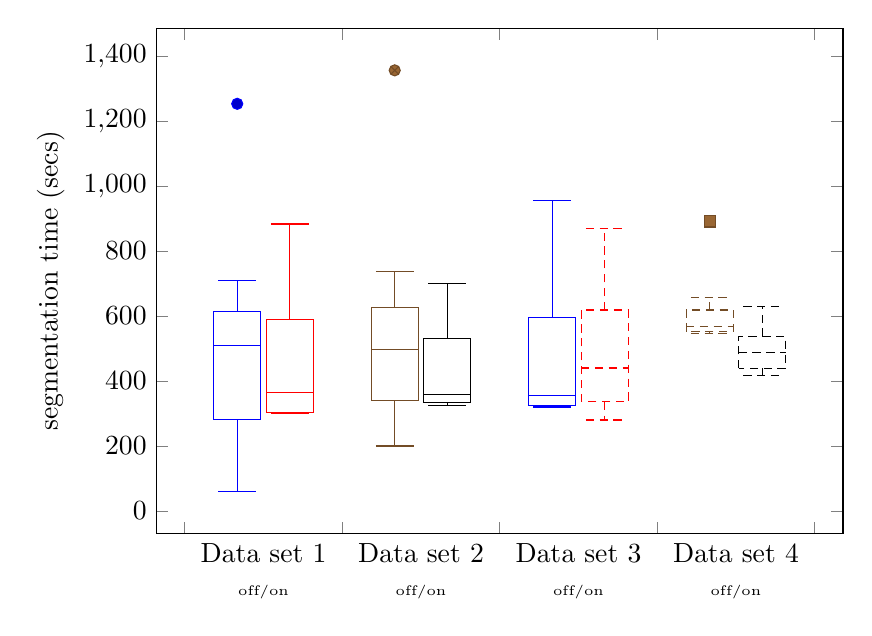
\begin{tikzpicture}
    \begin{axis}[
    boxplot/draw direction=y,
    ylabel={segmentation time (secs)},
    height=8cm,
    boxplot={
    	%
    	% Idea: 
    	%  place the 
    	%  group 1 at 0.3333 and 0.6666
    	%  group 2 at 1.3333 and 1.6666
    	%  group 3 at 2.3333 and 2.6666
    	%  ...
    	% in a formular:
    	draw position={1/3 + floor(\plotnumofactualtype/2) + 1/3*mod(\plotnumofactualtype,2)},
    	%
    	% that means the box extend must be at most 0.33333 :
    	box extend=0.3,
    },
    % ... it also means that 1 unit in x controls the width:
    x=2cm,
    % ... and it means that we should describe intervals:
    xtick={0,1,2,...,10},
    x tick label as interval,
    xticklabels={%
    	{Data set 1\\{\tiny off/on}},%
    	{Data set 2\\{\tiny off/on}},%
    	{Data set 3\\{\tiny off/on}},%
    	{Data set 4\\{\tiny off/on}},%
    },
        x tick label style={
            text width=2.5cm,
            align=center
        },
    ]
    
    \addplot
    table[row sep=\\,y index=0] {
    data\\
    60\\
    516\\
    710\\
    503\\
    1253\\
    };
    \addplot
    table[row sep=\\,y index=0] {
    data\\
    759\\
    419\\
    309\\
    883\\
    299\\
    };
    
    \addplot
    table[row sep=\\,y index=0] {
    data\\
    516\\
    480\\
    1356\\
    200\\
    736\\
    };
    \addplot
    table[row sep=\\,y index=0] {
    data\\
    684\\
    340\\
    700\\
    325\\
    377\\
    };
    
    \addplot
    table[row sep=\\,y index=0] {
    data\\
    956\\
    320\\
    811\\
    330\\
    381\\
    };
    \addplot
    table[row sep=\\,y index=0] {
    data\\
    280\\
    749\\
    392\\
    870\\
    488\\
    };
    
    \addplot
    table[row sep=\\,y index=0] {
    data\\
    658\\
    579\\
    891\\
    545\\
    558\\
    };
    \addplot
    table[row sep=\\,y index=0] {
    data\\
    514\\
    630\\
    416\\
    559\\
    462\\
    };
    
    \end{axis}
    \end{tikzpicture}
    
    
    \end{document}
